% !TeX root = ../dokumentation.tex

\chapter{Sprints}

\section{Sprint 1}
\todo{Beschreibung des Produktincrements}

\section{Ziele Sprint 1}
\todo{Ziel Sprint 1}

\section{Ergebnisse Sprint 1}

\subsection{Produktincrement}
\subsection{Charts}

\subsection{Probleme und Verbesserungen}
\todo{Retro Ergebnisse}


\subsection{Bearbeitete User Storys}

\subsubsection{Ticket 1}

\subsubsection{Ticket 2}

\subsubsection{SKIOS-59 Design Settings Interface}
Das Ticket \enquote{SKIOS-59 Design Settings Interface} hatte folgende User Story:
\begin{quotation}
    As a frontend developer, I would like to know how our settings interface should look so that I can start creating it.
    \textbf{The Mockup page should include:}
        \begin{itemize}
            \item A way to view and change the necessary settings
            \item An indication of what user is logged in
            \item A saving mechanism
        \end{itemize}
\end{quotation}
\textbf{Acceptance Criteria}
    \begin{itemize}
        \item Figma Mockups are designed for the settings page
        \item Mockups use existing components for articles, buttons and input fields
        \item Design uses SKIOSA colorscheme
        \item Design includes ways to change
        \begin{itemize}
            \item colorscheme
            \item language
            \item interest in categories
        \end{itemize}
        \item Design includes a link to changing password or to logout 
    \end{itemize}
Bearbeitet von Sophie Gösch.

\subsubsection{SKIOS-60 User Experience for Likes and Bookmarks}
Das Ticket \enquote{SKIOS-60 User Experience for Likes and Bookmarks} hatte folgende User Story:
\begin{quotation}
    As a ui/ux designer, I would like to know what a possible workflow for working with likes and bookmarks would be so that we can start implementing it.

    Possibly look up what User Experience Design is before working on this ticket \url{https://xd.adobe.com/ideas/career-tips/what-is-ux-design/}
\end{quotation}
\textbf{Acceptance Criteria}
    \begin{itemize}
        \item Definitions and Decisions are documented in confluence
        \item It is clear which pages to create for Bookmarks and Likes
        \item User Interaction with the side bar is clarified and a decision is made on where to place like or bookmark buttons
    \end{itemize}
\textbf{Ideas for a possible solution}
    \begin{itemize}
        \item Define Bookmarks in terms of our application (for reference see \URL{https://skiosa.atlassian.net/wiki/spaces/SKIOSA/pages/1015809/Draft+for+Project+Architecture} or \url{https://skiosa.atlassian.net/wiki/spaces/SKIOSA/pages/4063267/Epic+Drafts})
        \item Document findings in confluence under “UI/UX”
        \item Clarify how we should show users their bookmarks (in the side bar, in a sperate page), if a seperate page is chosen, think about where to place it (top level, nested under overview, nested under user pages, etc)
        \item Clarify if we need some type of read or watched like in youtube
        \item Clarify if Bookmarks work as marking of read bookmarks or of articles that you want to read in the future (and how this would impact how to structure bookmarks  ~ alphabetically, by unseen, let the recomendation engine use ML, etc)
        \item Should Likes also have an overview and how would they differ from Bookmarks
        \item Possibly decide if we even need bookmarks and likes or if one of them would be enough
        \item In Summary: define the where, what and how of bookmarks and likes
    \end{itemize}
Bearbeitet von Sophie Gösch.

\subsubsection{SKIOS-61 Design Subscription Interface}
Das Ticket \enquote{SKIOS-61 Design Subscription Interface} hatte folgende User Story:
\begin{quotation}
    As a frontend developer, I would like to know how our subscription interface should look so that I can start creating it.
    \textbf{The Mockup page should include:}
        \begin{itemize}
            \item A list of subscribed feeds (either up top or in seperate frame)
            \item A button or method to unsubscribe
            \item A list of most recent articles
            \item All other things that might be helpfull for a subscription page
        \end{itemize}
\end{quotation}
\textbf{Ideas for a possible solution}
    \begin{itemize}
        \item Use colorscheme and guidelines (see linked issues) to create pages
        \item For more information on the requirements for our user page see: \URL{https://skiosa.atlassian.net/wiki/spaces/SKIOSA/pages/4030475/Initial+Requirements} (might not be all too helpful in this case though)
        \item Possibly copy this page from youtube
    \end{itemize}
\textbf{Acceptance Criteria}
    \begin{itemize}
        \item Figma Mockups include subscription interface
        \item Interface includes the components named above
    \end{itemize}
Bearbeitet von Sophie Gösch.

/\subsubsection{SKIOS-62 Design Feed overview}
Das Ticket \enquote{SKIOS-62 Design Feed overview} hatte folgende User Story:
\begin{quotation}
    As a frontend developer, I would like to know how our feed overview interface should look so that I can start creating it.

    The feed overview is like the channel page in YouTube (ex. \url{https://www.youtube.com/channel/UC9m7D4XKPJqTPCLSBym3BCg/featured} ), just for RSS feeds.
    \textbf{The Mockup page should include:}
        \begin{itemize}
            \item Name of feed
            \item subscription status
            \item Recent articles
            \item possibly more information on feed
        \end{itemize}
\end{quotation}
\textbf{Ideas for a possible solution}
    \begin{itemize}
        \item Use colorscheme and guidelines (see linked issues) to create pages
        \item For more information on the requirements for our user page see: \URL{https://skiosa.atlassian.net/wiki/spaces/SKIOSA/pages/4030475/Initial+Requirements} (might not be all too helpful in this case though)
        \item Possibly copy this page from youtube
    \end{itemize}
\textbf{Acceptance Criteria}
    \begin{itemize}
        \item Figma Mockups include feed overview interface
        \item Interface includes the components named above
    \end{itemize}
Bearbeitet von Sophie Gösch.

\section{Sprint 2}
\subsection{Produktincrement}
\subsection{Charts}
\subsection{Probleme und Verbesserungen}


\subsection{Bearbeitete User Storys}

\subsubsection{SKIOS-69 Preliminary ORM}
Das Ticket \enquote{SKIOS-69 Preliminary ORM} hatte folgende User Story:
\begin{quotation}
    Als Programmierer will ich eine Datendefinition in einer Datenbank
    haben, und diese als Packet einbinden können.
\end{quotation}
Diese wurde folgendermaßen gelöst:
\begin{quotation}
Die Datendefinition wurde durch TypeORM~\parencite{web/TypeORM} dargestellt.
Diese wurde in dem Repository skiosa/orm~\parencite{git/skiosa/orm} als NPM-Package~\parencite{web/npm} abgebildet.
Es wurden die Article von RSS-Feeds in dem Schema aus Abbildung~\ref{fig:databaseORM} abgebildet.
\begin{figure}
    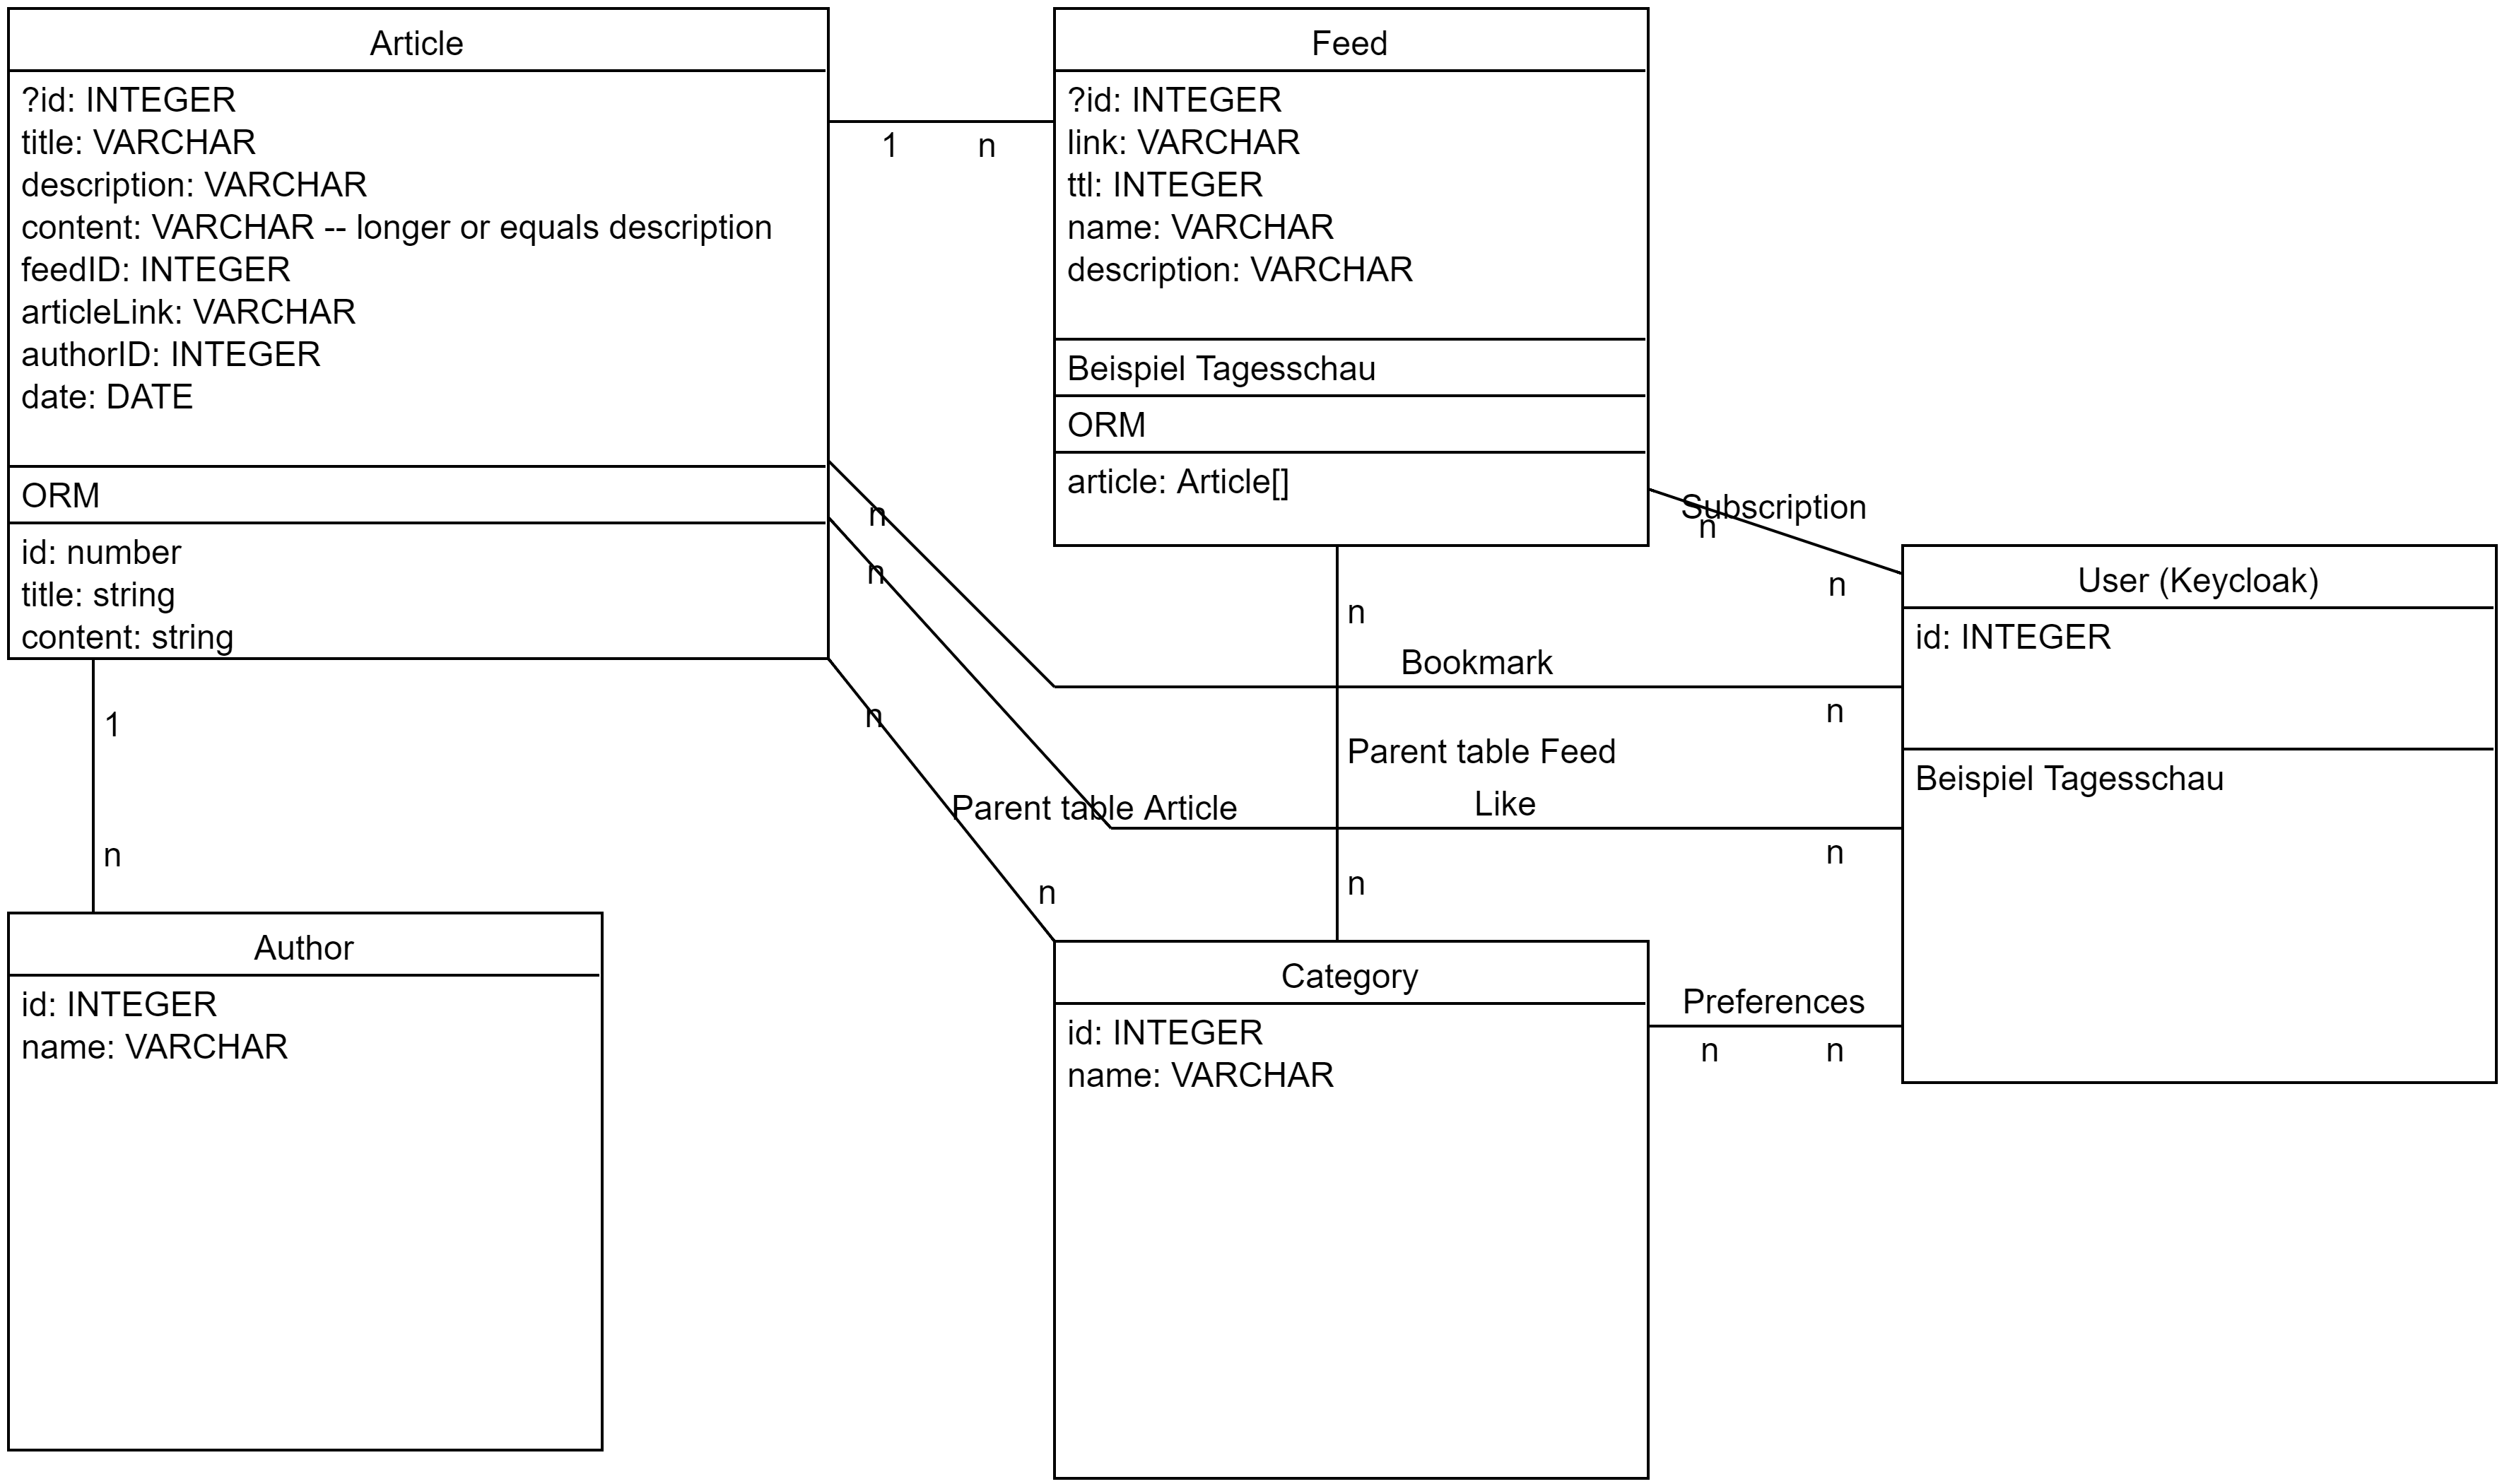
\includegraphics[width=\linewidth]{Database_Model.png}
    \caption{Datendefinition innerhalb der Datenbank}
    \label{fig:databaseORM}
\end{figure}
\end{quotation}
Bearbeitet von Jonas Eppard und Tim Horlacher.

\section{Sprint 3}

\subsection{Produktincrement}
\subsection{Charts}
\subsection{Probleme und Verbesserungen}


\subsection{Bearbeitete User Storys}
\subsubsection{SKIOS-116 Structure and table of contents for submission (\LaTeX)}
Das Ticket \enquote{SKIOS-116 Structure and table of contents for submission (\LaTeX)}
hatte folgende User Story:
\begin{quotation}
    As a team member, I would like to have a rough structure to orient myself while writing our submission documentation.\\
    For this story, please read the requirements and guidelines set out by Garidis and develop a rough idea on how to structure our \LaTeX project.\\
    \textbf{Acceptance Criteria}
    \begin{itemize}
        \item Table of contents is created (with \textbackslash{}section, \textbackslash{}subsection, etc.) in \LaTeX
        \item Structure reflects guidelines of Garidis
        \item Structure is explained in confluence page
        \item Existing \LaTeX~stories have a defined place where their pages will go
    \end{itemize}
\end{quotation}
Dies wurde folgendermaßen gelöst:
\begin{quotation}
    Es wurde die Struktur dieses \LaTeX-Dokuments angelegt. Hierbei musste nur das Inhaltsverzeichnis
    angelegt werden, da das \LaTeX-Template schon vorhanden war.
    Die Verwendung wurde in Confluence dokumentiert.
\end{quotation}
Bearbeitet von Jonas Eppard.

\section{Sprint 4}
\todo{Beschreibung des Produktincrements}

\section{Ziele Sprint 4}
\todo{Ziel Sprint 4}

\section{Ergebnisse Sprint 4}

\subsection{Produktincrement}
\subsection{Charts}

\subsection{Probleme und Verbesserungen}
\todo{Retro Ergebnisse}


\subsection{Bearbeitete User Storys}

\subsubsection{SKIOS-152 LaTeX Sprint Summaries}
Das Ticket \enquote{SKIOS-152 LaTeX Sprint Summaries} hatte folgende User Story:
\begin{quotation}
    As a member of this team, I would like to have each sprint explained in our Sprints chapter.
    \textbf{Goal of this story is to fill out the parts for:}
        \begin{itemize}
            \item “Ziele Sprint XY”
            \item “Ergebnisse Sprint XY”
            \item “Produktinkrement”
            \item if referenced in other sections: “Charts”
            \item “Probleme und Verbesserungen”
        \end{itemize}
        für jeden Sprint
\end{quotation}
\textbf{Acceptance Criteria}
    \begin{itemize}
        \item LaTeX Pages are created
        \item “Ziele Sprint XY” and “Produktincrement” are discussed with PO
        \item “Probleme und Verbesserungen” lists and discusses results of Retros
        \item Charts section is only created if referenced in any other part of this documentation
        \item A quick summary is created at the top of each sprint including:
        \begin{itemize}
            \item Timeline of the sprint
            \item Meetings of that sprint and dates for them (Bi weekly, weekly, review, retro, estimation meetings) => See (incomplete) meeting notes
            \item Capacity for that sprint
        \end{itemize}
        \item Page is spellchecked
    \end{itemize}
Bearbeitet von Sophie Gösch.